\section{Tekstanalyse}
På Android kan man få adgang til SMS beskeder og disse kan derefter analyseres til at finde ud af en persons sindsstilling. Det kræver rettighed til applikationen til at læse SMS'er, og man skal derfor overveje brugerens privatliv. 

Data er SMS beskeder, d.v.s. en mængde af ustrukturerede tekster med tilknyttet metadata, såsom afsendelsestidspunkt og modtager.

\subsection{Antal, nøgleord og andre metadata}
Man kan konstruere data som antal beskeder brugeren modtager, og om der er nogle specifikke nøgleord som kunne være interessante fra et psykiatrisk synspunkt. F.eks. kan man se om de bruger ordet "deprimeret", om de bruger positivt eller negativt ladede ord, eller om der bruges korte eller lange ord. 

Andre metadata som afsendelsestidspunkt, modtager, respons kan også være interessante at kigge på og disse kan også nemt udtrækkes \citep{misc:androidsmsread}.

Afsendelsestidspunkt kunne e.v.t. være interessant til at se om sindstilstand er kontinuert, således at man kan se om en negativ ladet sms tekst er vedvarende over en længere periode eller om det er et enkeltstående tilfælde.
		
Modtager kunne være interessant til at se, om man til personer man normalt har en ensformig tekst stemning mod, ændrer sig til eksempelvis meget negativt ladede tekster.

Længden af SMSerne kan bruges til at registere adfærdsændringer, eksempelvis en person der typisk har SMS'er med en længde på 10 ord i gennemsnit pludselig får et gennemsnit på 30+ ord.


\subsection{Sentiment analysis}
Hvis man skal lave sentiment analysis kræver det en stor mængde af træningsdata, for at tekstanalysen bliver akkurat. Twitter kunne evt. være en ressource til at finde sådanne data. Problemet er at det skal være på dansk, og er nok her en stor del af arbejdet med sentiment analysis af danske SMS tekster ligger.
Det vil være selve SMS teksterne der er centrale i tekstanalyse når det kommer til sentiment analysis. 
Hvis denne kan gøres præcis kunne man få en meget god indikation på en brugers sindsstilling.

\begin{comment}
Til dette skulle man bruge træningsdata som kan bruges til at opbygge en sentiment analysis classifier, eksempelvis Naïve Bayes Classifier. Denne classifier vil så kunne bruges til at vurdere sindstilstand for brugere. Hvis træningsdata ikke er tilgængeligt kunne man se på negative eller positive ord og hvordan de bruges i SMS teksten.

\end{comment}

\subsection{Visualisering}
Man kunne bruge disse til at få et øjebliksbillede som kunne vises til brugeren eller brugerens psykiater/psykolog i form af en beskrivende besked om sindstilstand, evt. med tal for hvor sikker vi er på denne bedømmelse. Her forstilles det en skala over sindstilstande, hvor forskellige niveauer har en tilhørende beskrivelse.
Hvis man skulle tage analysen i et kronologisk perspektiv kunne en graf med tid og sindstilstandsniveau være en mulighed. 

\begin{figure}
	\centering
	\begin{subfigure}[b]{0.3\textwidth}
		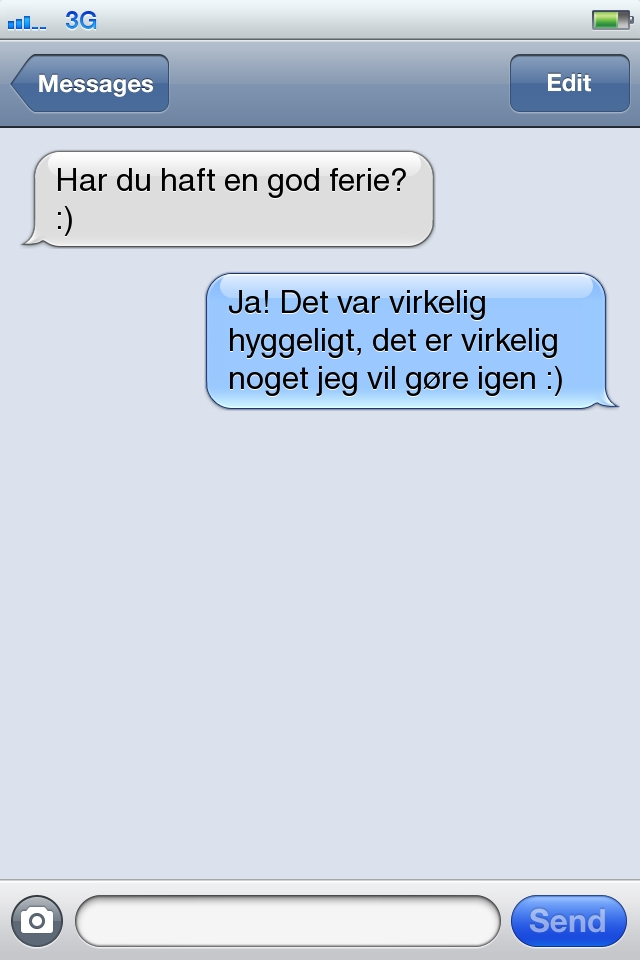
\includegraphics[width=\textwidth]{positiveSMS}
		\caption{Positiv SMS}
	\end{subfigure}
	~
	\begin{subfigure}[b]{0.3\textwidth}
		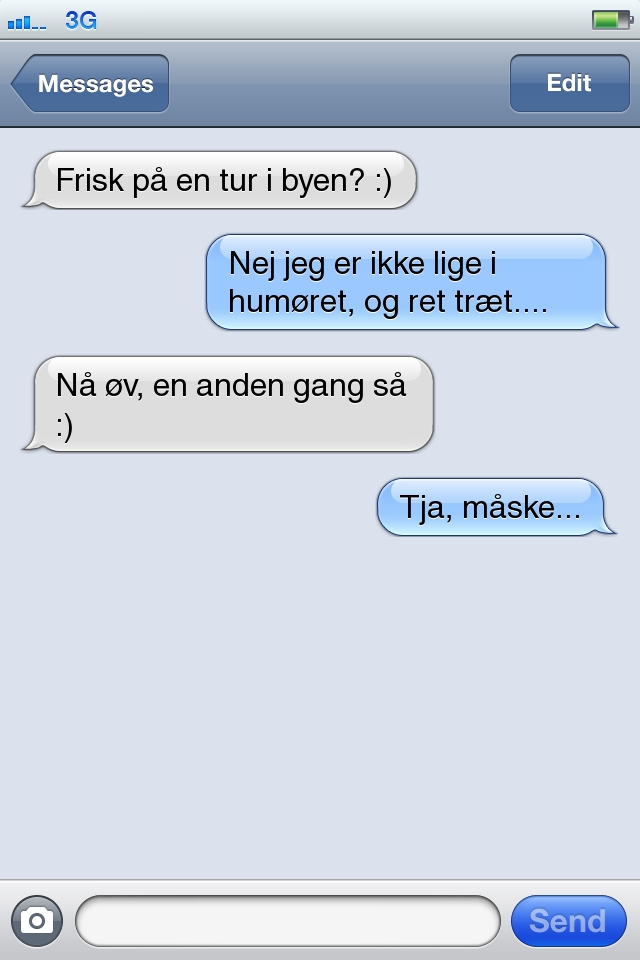
\includegraphics[width=\textwidth]{negativeSMS}
		\caption{Negativ SMS}
	\end{subfigure}
	\caption{Eksempler på SMS'er}
\end{figure}
	
	